% !TeX root = ActuarialFormSheet_MBFA_MPG.tex
% !TeX spellcheck = fr_FR

\begin{f}[Pythagore]
Dans un triangle rectangle, le carré de l’hypoténuse est égal à la somme des carrés des deux autres côtés. Si \(ABC\)  est rectangle en \(C\), alors 

%
\begin{tikzpicture}[scale=.85]
	% Triangle
	\coordinate [label=above left:\(C\)] (C) at (0,0);
	\coordinate [label=above right:\(B\)] (B) at (4,0);
	\coordinate [label=below left:\(A\)] (A) at (0,3);
	
	%\draw[thick] (A) -- (B) -- (C) -- cycle;
	
	% Carré sur AC
	\draw[BleuProfondIRA!60] (A) -- (C) ;
	\node at (-0.6,1.5) {\color{BleuProfondIRA}\(AC^2\)};
	
	% Carré sur BC
	\draw[VertIRA] (B) -- (C);
	\node at (2,0.6) {\color{VertIRA}\(BC^2\)};
	
	% Carré sur AB
	\draw[OrangeProfondIRA] (A) -- (B) ;
	\node at (2.5,1.75) {\color{OrangeProfondIRA}\(AB^2\)};
	
	% Angle droit
	\draw (C) rectangle +(0.3,0.3);
	\node[right] at (3.75,1.75) {\(
		\color{OrangeProfondIRA}AB^2 = \color{VertIRA}AC^2 +\color{BleuProfondIRA} BC^2
		\)};
\end{tikzpicture}
\end{f}

\begin{f}[Thalès]
Soient deux droites \textbf{sécantes en un point} \( A \), et soient deux droites \( (BC) \) et \( (DE) \) \textbf{parallèles}, coupant les deux droites en \( B, D \) et \( C, E \), alors :
\[
\frac{AB}{AD} = \frac{AC}{AE} = \frac{BC}{DE}
\]


\begin{center}
	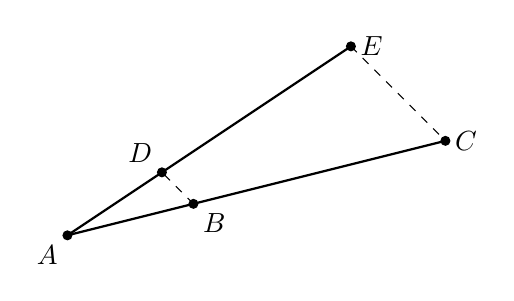
\begin{tikzpicture}[scale=.8]
		% Points
		\coordinate (A) at (0,0);
		\coordinate (B) at (2,0.5);
		\coordinate (C) at (6,1.5);
		\coordinate (D) at (1.5,1);
		\coordinate (E) at (4.5,3);
		
		% Segments
		\draw[thick] (A) -- (C);
		\draw[thick] (A) -- (E);
%		\draw[thick] (B) -- (C);
%		\draw[thick] (D) -- (E);
		\draw[dashed] (B) -- (D);
		\draw[dashed] (E) -- (C);
		
		% Points
		\filldraw[black] (A) circle (2pt) node[below left] {\(A\)};
		\filldraw[black] (B) circle (2pt) node[below right] {\(B\)};
		\filldraw[black] (C) circle (2pt) node[right] {\(C\)};
		\filldraw[black] (D) circle (2pt) node[above left] {\(D\)};
		\filldraw[black] (E) circle (2pt) node[right] {\(E\)};
		
%		% Parallèles
%		\draw[<->,blue,thick] (0.8,2.2) -- (3.2,2.2) node[right] {\small \(\ell\)};
%		\draw[<->,blue,thick] (0.8,0.8) -- (3.2,0.8) node[right] {\small \(\ell'\)};
%		\node at (3.6,1.5) {\small \(\ell \parallel \ell'\)};
	\end{tikzpicture}
\end{center}
\end{f}
\hrule

\begin{f} [Équation du second degré] 
     \[
    ax^2 + bx + c = 0
    \]

    Le discriminant est défini par :
    
    \[
    \Delta = b^2 - 4ac
    \]
       
    \begin{itemize}
        \item Si \(\Delta > 0\), l'équation a deux solutions distinctes :
        \[
        x_1 = \frac{-b + \sqrt{\Delta}}{2a}, \quad x_2 = \frac{-b - \sqrt{\Delta}}{2a}
        \]
        \item Si \(\Delta = 0\), l'équation a une solution double :
        \[
        x = \frac{-b}{2a}
        \]
        \item Si \(\Delta < 0\), l'équation a une solution dans les imaginaires
        \[
        x_1 = \frac{-b + i\sqrt{\Delta}}{2a}, \quad x_2 = \frac{-b - i\sqrt{\Delta}}{2a}
        \]
    \end{itemize}
\end{f}
\hrule
\begin{f} [Fonctions factorielle, dénombrement et Gamma] 

La fonction \textbf{factorielle} (de \(\mathbb{N}\) dans \(\mathbb{N}\) ) est définie par \(0!=1\) et \(n!=n \times(n-1) \times \cdots \times 2 \times 1=\) permutations de \(n\) éléments \(\displaystyle C_n^k=\binom{k}{n}=\frac{n!}{k!(n-k)!}=\) choix de \(k\) éléments parmi \(n\) les \(C_n^k\) se calculent aussi par le triangle de Pascal et vérifient:

\[
C_n^k=C_n^{n-k}, C_n^k+C_n^{k+1}=C_{n+1}^{k+1} .
\]


Soit \(E\) un ensemble de cardinal \(\operatorname{Card}(E)\) et de parties \(\mathcal{P}(E)\) :

\[
\begin{aligned}
\operatorname{Card}(\mathcal{P}(E)) & =2^{\operatorname{Card}(E)} \\
\operatorname{Card}(A \times B) & =\operatorname{Card}(A) \times \operatorname{Card}(B) \\
\operatorname{Card}(A \cup B) & =\operatorname{Card}(A)+\operatorname{Card}(B)-\operatorname{Card}(A \cap B)
\end{aligned}
\]
\[ \Gamma(n) = \int_0^\infty t^{n-1} e^{-t} \, dt \]
La fonction \(\Gamma\) peut être vue comme le prolongement de la factorielle : \(\Gamma(n+1)=n!\).
\end{f}

\hrule
\begin{f}
	[Développement binomial] 
	
	Pour un entier positif \(n\),
	\[
	(x+y)^n=\sum_{i=0}^n\binom{n}{i} x^i y^{n-i}
	\]
	
\end{f}
\hrule
\begin{f}[Suites]  
	
	Les suites arithmétiques de raison \(r\)
	
	\[
	\left\{\begin{array} { r l } 
		{ u _ { n + 1 } } & { = u _ { n } + r } \\
		{ u _ { 0 } } & { \in \mathbb { R } }
	\end{array} \Rightarrow \left\{\begin{array}{rl}
		u_n & =n r+u_0 \\
		\sum_{k=0}^n u_k & =\frac{(n+1)\left(2 u_0+n r\right)}{2}
	\end{array}\right.\right.
	\]
	
	suites géométriques de raison \(q\left\{\begin{array}{rll}u_{n+1} & = & q \times u_n \\ u_0 & \in & \mathbb{R}\end{array}\right.\)
	
	\[
	\Rightarrow\left\{\begin{array}{rlr}
		u_n & =u_0 \times q^n \\
		\sum_{k=0}^n u_k & =\left\{\begin{array}{rl}
			(n+1) u_0 & \text { si } \\
			u_0 \frac{1-q^{n+1}}{1-q} & \text { sinon }
		\end{array} \quad q=1\right.
	\end{array}\right.
	\]
	
\end{f}
\hrule
\begin{f}[Exponentielle et Logarithme]
	La fonction exponentielle \( e^x \) peut être définie par le développement en série entière suivant :
	
	\[
	e^x = \sum_{n=0}^{\infty} \frac{x^n}{n!} = 1 + x + \frac{x^2}{2!} + \frac{x^3}{3!} + \cdots
	\]
	
	Cette série converge pour tout \( x \in \mathbb{R} \) et permet de définir l'exponentielle comme une somme infinie.
	
	
	La fonction logarithme naturel \( \ln(x) \) est définie comme la primitive de la fonction \( \frac{1}{x} \). Autrement dit :
	
	\[
	\frac{d}{dx} \ln(x) = \frac{1}{x}
	\]
	
	avec la condition \( \ln(1) = 0 \). Cette définition permet d'établir le lien entre l'exponentielle et le logarithme via l'inversion : \( e^{\ln(x)} = x \) pour \( x > 0 \).
	
\end{f}



\hrule
\begin{f}[Relation de congruence]
	Soit \(m > 0\). On dit que deux réels \(a\) et \(b\) sont congrus modulo \(m\) s'il existe un entier relatif \(k \in \mathbb{Z}\) tel que :
	\[
	a = b + km.
	\]
	On note \(a \equiv b \pmod{m}\).
	
	En trigonométrie, on choisit souvent \(m = 2\pi\) ou \(m = \pi\).
\end{f}

\begin{f}
	[Cercle trigonométrique — sinus, cosinus, tangente]
	
		\begin{animateinline}[poster=first, autoplay,loop]{1}
			\multiframe{24}{i=0+1}{%
				\begin{tikzpicture}[scale=3,yrange=-4:4]
\node[text width=9cm, align=left] at (0,3.75) {\ \(\displaystyle M = (\cos \theta, \sin \theta)\)};
\node[text width=9cm, align=left] at (0,3.5) {\ Si \(\theta \not\equiv \frac{\pi}{2} \pmod{\pi}\), on définit :
	\(\displaystyle
	\tan \theta = \frac{\sin \theta}{\cos \theta}
	\)};
\node[text width=9cm, align=left] at (0,3.25) {\ \(\displaystyle \cos^2 \theta + \sin^2 \theta = 1 \)};
\node[text width=9cm, align=left] at (0,2.5) {\renewcommand{\arraystretch}{1.5}\begin{tabular}{|c|c|c|c|c|c|}
		\hline\rowcolor{BleuProfondIRA!40}
		\(\theta\) & \(0\) & \(\frac{\pi}{6}\) & \(\frac{\pi}{4}\) & \(\frac{\pi}{3}\) & \(\frac{\pi}{2}\) \\
		\hline
		\(\cos \theta\) & \(1\) & \(\frac{\sqrt{3}}{2}\) & \(\frac{\sqrt{2}}{2}\) & \(\frac{1}{2}\) & \(0\) \\
		\hline
		\(\sin \theta\) & \(0\) & \(\frac{1}{2}\) & \(\frac{\sqrt{2}}{2}\) & \(\frac{\sqrt{3}}{2}\) & \(1\) \\
		\hline
		\(\tan \theta\) & \(0\) & \(\frac{\sqrt{3}}{3}\) & \(1\) & \(\sqrt{3}\) & indéfini \\
		\hline
\end{tabular}};
\node[text width=9cm, align=left] at (0,-2.75) {\small\renewcommand{\arraystretch}{1.5}	
\begin{tabular}{|c|c|c|}
	\hline\rowcolor{BleuProfondIRA!40}
	\(-\theta\) & \(\theta + \pi\) & \(\pi - \theta\) \\
	\hline
	\(\cos \theta\) & \(-\cos \theta\) & \(-\cos \theta\) \\
	\hline
	\(-\sin \theta\) & \(-\sin \theta\) & \(\sin \theta\) \\
	\hline
	\hline\rowcolor{BleuProfondIRA!40}
	\(\theta + 2\pi\) & \(\frac{\pi}{2} - \theta\) & \(\frac{\pi}{2} + \theta\) \\
	\hline
	\(\cos \theta\) & \(\sin \theta\) & \(-\sin \theta\) \\
	\hline
	\(\sin \theta\) & \(\cos \theta\) & \(\cos \theta\) \\
	\hline
\end{tabular}
 \\ \vspace{2mm}
\ \(\cos x = \cos y \iff \begin{cases}
	x \equiv y \pmod{2\pi} \text{ ou }\\ x \equiv -y \pmod{2\pi}
\end{cases} \) \\
\ \(\sin x = \sin y \iff \begin{cases}
	 x \equiv y \pmod{2\pi} \text{ ou }\\ x \equiv \pi - y \pmod{2\pi}
\end{cases}\)\\
\ \(\tan x = \tan y \iff x \equiv y \pmod{\pi}\)
};


	\def\radius{1}
	\pgfmathsetmacro{\angle}{15*\i+45} % degr\'es
	\pgfmathsetmacro{\cosx}{cos(\angle)}
	\pgfmathsetmacro{\siny}{sin(\angle)}
	
	% Coordonn\'ees de M
	\coordinate (M) at ({\cosx}, {\siny});
	
	% Axes
	\draw[->] (-0.2,0) -- (1.25,0) node[anchor=west] {\(x\)};
	\draw[->] (0,-1.5) -- (0,1.25) node[anchor=south] {\(y\)};
	
	% Cercle
	\draw[thick] (0,0) circle(\radius);
	
	% OM
	\draw[->, thick, BleuProfondIRA] (0,0) -- (M) node[above right] {\(M\)};
	
	% Projections cosinus et sinus
	\draw[dashed] (M) -- ({\cosx}, 0);
	\draw[dashed] (M) -- (0, {\siny});
	
	\draw[<->, thick, OrangeProfondIRA] (0, -0.1) -- ({\cosx}, -0.1);
	\node[below, OrangeProfondIRA] at ({\cosx/2}, -0.1) {\(\cos\theta\)};
	
	\draw[<->, thick, VertIRA] (-0.1, 0) -- (-0.1, {\siny});
	\node[left, VertIRA] at (-0.1, {\siny/2}) {\(\sin\theta\)};
	
	% Angle
	\draw[->, FushiaIRA] (0.5,0) arc[start angle=0, end angle=\angle, radius=0.5];
	\node at (0.7,0.15) {\(\theta\)};
	
	% Tangente (affich\'ee sauf si angle = 90\textdegree{} ou 270\textdegree{})
	\pgfmathtruncatemacro{\angleInt}{\angle} % angle en entier
	\ifnum\angleInt=90
	\draw[dashed] (1,-4) -- (1,4);
	\node[right] at (1,1.3) {\(x=1\)};
	\else\ifnum\angleInt=270
	\draw[dashed] (1,-4) -- (1,4);
	\node[right] at (1,1.3) {\(x=1\)};
	\else
	\pgfmathsetmacro{\tany}{tan(\angle)}
	\draw[dashed, gray] (0,0) -- (1.05, {\tany*1.05});
	\draw[dashed] (1,-4) -- (1,4);
	\coordinate (T) at (1, {\tany});
	\draw[fill=black] (T) circle(0.015);
	\node[above right] at (T) {\(T\)};
	\node[below right] at (T) {\((1,\tan\theta)\)};
	\node[right] at (1,1.3) {\(x=1\)};
	\fi\fi
\end{tikzpicture}
			}%
		\end{animateinline}
	
\end{f}
\renewcommand{\arraystretch}{1}

\columnbreak
\begin{f}
	[Propriétés de la relation de congruence]
	
	Soient \(m > 0\) et \(a, b, c, d \in \mathbb{R}\). Alors :
	
	\begin{itemize}
		\item \textbf{Réflexivité} : \(a \equiv a \pmod{m}\).
		\item \textbf{Symétrie} : \(a \equiv b \pmod{m} \iff b \equiv a \pmod{m}\).
		\item \textbf{Transitivité} : si \(a \equiv b \pmod{m}\) et \(b \equiv c \pmod{m}\), alors \(a \equiv c \pmod{m}\).
		\item \textbf{Additivité} : si \(a \equiv b \pmod{m}\) et \(c \equiv d \pmod{m}\), alors \(a + c \equiv b + d \pmod{m}\).
	\end{itemize}
	
\end{f}	

\hrule
\begin{f}[Dérivées et primitives] 

\[
\begin{aligned}
& f \text { continue en } x_\mathrm{m} \Leftrightarrow \lim _{x \rightarrow x_\mathrm{m}} f(x)=f\left(x_\mathrm{m}\right) \\
& f \text { dérivable en } x_\mathrm{m} \Leftrightarrow \exists \lim _{h \rightarrow 0} \frac{f\left(x_\mathrm{m}+h\right)-f\left(x_\mathrm{m}\right)}{h}=: f^{\prime}\left(x_\mathrm{m}\right)
\end{aligned}
\]
 
L'\textbf{intégrale de Riemann} d'une fonction \( f(x) \) sur un intervalle \([a, b]\) est la limite, si elle existe, de la somme des aires des rectangles approchant l'aire sous la courbe, donnée par :  

\[
\int_a^b f(x) \, dx = \lim_{n \to \infty} \sum_{i=1}^n f(x_i^*) \Delta x_i,
\]
\begin{itemize}
\item \( [x_{i-1}, x_i] \) est une subdivision de \([a, b]\),  
\item \( \Delta x_i = x_i - x_{i-1} \) est la largeur du sous-intervalle,  
\item \( x_i^* \in [x_{i-1}, x_i] \) est un point choisi arbitrairement dans chaque sous-intervalle.
\end{itemize}
  
\newcounter{numberofdiscretisation} \setcounter{numberofdiscretisation}{1}
\begin{center}
	    \begin{animateinline}[autoplay,loop,poster=15]{2}
      \whiledo{\thenumberofdiscretisation<20}{
        \begin{tikzpicture}[line cap=round, line join=round, >=triangle 45,
                            x=2.6cm, y=1.0cm, scale=1]
           \draw [->,color=OrangeProfondIRA] (-0.1,0) -- (2.5,0);
          \foreach \x in {1,2}
            \draw [shift={(\x,0)}, color=OrangeProfondIRA] (0pt,2pt)
                  -- (0pt,-2pt) node [below] {\footnotesize \(\x\)};
          \draw [color=OrangeProfondIRA] (2.5,0) node [below] {\(x\)};
          \draw [->,color=OrangeProfondIRA] (0,-0.1) -- (0,4.5);
          \foreach \y in {1,2,3,4}
            \draw [shift={(0,\y)}, color=OrangeProfondIRA] (2pt,0pt)
                  -- (-2pt,0pt) node[left] {\footnotesize \(\y\)};
          \draw [color=OrangeProfondIRA] (0,4.5) node [right] {\(y\)};
          \draw [color=OrangeProfondIRA] (0pt,-10pt) node [left] {\footnotesize \(0\)};
          \draw [color=OrangeProfondIRA, domain=0:2.2, line width=1.0pt] plot (\x,{(\x)^2});
          \clip(0,-0.5) rectangle (3,5);
          \draw (2,0) -- (2,4);
          \foreach \i in {1,...,\thenumberofdiscretisation}
            \draw [draw=BleuProfondIRA,fill=BleuProfondIRA,fill opacity=0.3, smooth,samples=50] ({1+(\i-1)/\thenumberofdiscretisation},{(1+(\i)/\thenumberofdiscretisation)^2})
                  --({1+(\i)/\thenumberofdiscretisation},{(1+(\i)/\thenumberofdiscretisation)^2})
                  --  ({1+(\i)/\thenumberofdiscretisation},0)
                  -- ({1+(\i-1)/\thenumberofdiscretisation},0)
                  -- cycle;
        \end{tikzpicture}
        %
        \stepcounter{numberofdiscretisation}
        \ifthenelse{\thenumberofdiscretisation<20}{ \newframe }{\end{animateinline} }
      }
      
\end{center}
      Exemple d'intégrale de Riemann (upper)\href{https://texample.net/media/tikz/examples/TEX/upper-riemann-sum.tex}{\(^*\)}
 
 

L'\textbf{intégrale de Lebesgue} d'une fonction \( f(x) \) sur un ensemble \( E \) est définie en mesurant l'aire sous la courbe en fonction des valeurs prises par \( f \), donnée par :  
\[
\int_E f \, d\mu = \int_0^\infty \mu(\{x \in E : f(x) > t\}) \, dt,
\]
\begin{itemize}
    \item \( \mu \) est une mesure (souvent la mesure de Lebesgue),  
\item \( \{x \in E : f(x) > t\} \) représente l'ensemble des points où \( f(x) \) dépasse \( t \).  
\end{itemize} 
À la différence de Riemann, Lebesgue regroupe les points selon leurs valeurs plutôt que selon leur position.

\renewcommand{\arraystretch}{1.5}
\[
\begin{array}{|c|c|c|}
\hline \rowcolor{BleuProfondIRA!40} \text { fonction }(n \in \mathbb{R}) & \text { dérivée } & \text { primitive } \\
\hline x & 1 & \frac{x^2}{2}+C \\
\hline x^2 & 2 x & \frac{x^3}{3}+C \\
\hline 1 / x & -1 / x^2 & \ln (x)+C \\
\hline \sqrt{x}=x^{1 / 2} & \frac{1}{2 \sqrt{x}} & \frac{2}{3} x^{3 / 2}+C \\
\hline x^n, n \neq-1 & n x^{n-1} & \frac{x^{n+1}}{n+1}+C \\
\hline \ln (x) & 1 / x & x \ln (x)-x+C \\
\hline e^x & e^x & e^x+C \\
\hline a^x=e^{x \ln (a)} & \ln (a) \times a^x & a^x / \ln (a)+C \\
\hline \sin (x) & \cos (x) & -\cos (x)+C \\
\hline \cos (x) & -\sin (x) & \sin (x)+C \\
\hline \tan (x) & 1+\tan (x) & -\ln (|\cos (x)|)+C \\
\hline 1 /\left(1+x^2\right) & -2 x /\left(1+x^2\right)^2 & \arctan (x)+C \\
\hline
\end{array}
\]
\renewcommand{\arraystretch}{1}

\[
    \begin{array}{rl|rl}
(u+v)^{\prime} & =u^{\prime}+v^{\prime} & \left(\frac{1}{u}\right)^{\prime} & =-\frac{u^{\prime}}{u^2} \\
(k u)^{\prime} & =k u^{\prime} & (\ln (u))^{\prime} & =\frac{u^{\prime}}{u} \\
(u \times v)^{\prime} & =u^{\prime} v+u v^{\prime} & (\exp (u))^{\prime} & =\exp (u) \times u^{\prime} \\
\left(\frac{u}{v}\right)^{\prime} & =\frac{u^{\prime} v-u v^{\prime}}{v^2} & (f(u))^{\prime} & =f^{\prime}(u) \times u^{\prime} \\
\left(u^n\right)^{\prime} & =n u^{n-1} \times u^{\prime} & (f \circ u)^{\prime} & =\left(f^{\prime} \circ u\right) \times u^{\prime}
\end{array}
\]
\end{f}

\hrule

\begin{f} [Intégration par parties] 

Soit \( u(x) \) et \( v(x) \) deux fonctions continûment dérivables sur l'intervalle \([a, b]\), alors

\[
\int_a^b u(x) v'(x) \, dx = \left[ u(x) v(x) \right]_a^b - \int_a^b u'(x) v(x) \, dx
\]

où :
\begin{itemize}
    \item \( u(x) \) est une fonction dont on connaît la dérivée \( u'(x) \),
    \item \( v'(x) \) est une fonction dont on connaît la primitive \( v(x) \).
\end{itemize}

\end{f}
\hrule
\begin{f}[Intégration avec changement de variable] 

Soit \( f(x) \) une fonction continue et \( x = \phi(t) \) un changement de variable, où \( \phi \) est une fonction dérivable. Alors :

\[
\int_{a}^{b} f(x) \, dx = \int_{\phi^{-1}(a)}^{\phi^{-1}(b)} f(\phi(t)) \phi'(t) \, dt
\]

où :
\begin{itemize}
    \item \( x = \phi(t) \) représente le changement de variable,
    \item \( \phi'(t) \) est la dérivée de \( \phi(t) \),
    \item les bornes de l'intégrale sont ajustées en fonction du changement de variable.
\end{itemize}
\end{f}

\hrule
\begin{f}
 [Formule de Taylor] 
 
Soit \( f(x) \) une fonction \( n \) - fois dérivable en un point \( a \). Le développement de Taylor de \( f(x) \) autour de \( a \) est donné par :

\begin{align*}
 f(x) =& f(a) + f'(a)(x - a) + \frac{f''(a)}{2!}(x - a)^2 \\
 &+ \cdots + \frac{f^{(n)}(a)}{n!}(x - a)^n + \mathcal{O}_n(x)
\end{align*}


où :
\begin{itemize}
    \item \( f^{(n)}(a) \) est la \( n \)\ieme{} dérivée de \( f \) évaluée en \( a \),
    \item \( \mathcal{O}_n(x) \) est le reste du développement de Taylor, représentant l'erreur d'approximation lorsque l'on tronque la série après le terme d'ordre \( n \), avec 
    \[
    \lim_{x\rightarrow 0}\frac{\mathcal{O}_n(x) }{x^n}\Rightarrow 0
    \]
\end{itemize}
\end{f}
\hrule
\begin{f}[Théorème des valeurs intermédiaires] 

Soit \( f \) une fonction continue sur un intervalle fermé \([a, b]\) et \( f(a) \neq f(b) \). Le théorème des valeurs intermédiaires affirme que pour tout réel \( c \) compris entre \( f(a) \) et \( f(b) \), il existe un point \( x \in [a, b] \) tel que :

\[
f(x) = c
\]

Autrement dit, si une fonction est continue sur un intervalle, elle prend toutes les valeurs comprises entre \( f(a) \) et \( f(b) \) au moins une fois.
\end{f}
\hrule
\begin{f}[Matrices et propriétés]
  
\textbf{Matrices diagonales :}
Une matrice est dite diagonale si tous les éléments en dehors de la diagonale principale sont nuls. Pour une matrice \( A \in \mathbb{R}^{n \times n} \), cela s'écrit :
\[
A = \text{diag}(a_1, a_2, \dots, a_n)
\]
où \( a_i \) sont les éléments diagonaux.

\textbf{Matrices triangulaires :}
Une matrice est triangulaire supérieure si tous les éléments en dessous de la diagonale sont nuls, c'est-à-dire \( A_{ij} = 0 \) pour \( i > j \). Inversement, elle est triangulaire inférieure si \( A_{ij} = 0 \) pour \( i < j \).
\end{f}
\begin{f}[Déterminant d'une matrice]
  
Le déterminant d'une matrice carrée \( A \in \mathbb{R}^{n \times n} \) est un scalaire, noté \( \det(A) \) :
\begin{itemize}
    \item Si \( A \) est une matrice carrée \( n \times n \), alors \( A \) est inversible si et seulement si \( \det(A) \neq 0 \).
    \item Le déterminant d'une matrice triangulaire (supérieure ou inférieure) ou d'une matrice diagonale :
    \[
    \det(A) = \prod_{i=1}^{n} A_{ii}
    \]
    \item
    \[
    \det(AB) = \det(A) \cdot \det(B),\quad \det(\lambda B) = \lambda\det(B), 
    \]
    \item 
    \[
    \det(A^T) = \det(A)
    \]
    \item Si une matrice \( A \) contient deux lignes ou colonnes identiques, alors \( \det(A) = 0 \).
\end{itemize}

\textbf{Calcul du déterminant :}
Le déterminant d'une matrice \( 2 \times 2 \) se calcule simplement par :
\[
\det\begin{pmatrix} a & b \\ c & d \end{pmatrix} = ad - bc
\]
Pour une matrice \( 3 \times 3 \), il est donné par :
\[
\det\begin{pmatrix} a & b & c \\ d & e & f \\ g & h & i \end{pmatrix} = a(ei - fh) - b(di - fg) + c(dh - eg)
\]
Pour des matrices de dimension supérieure, le déterminant peut être calculé par cofacteurs ou via une méthode de réduction (par exemple, la méthode de Gauss).

\end{f}
\hrule
\begin{f}[Inversibilité d'une matrice] 
Une matrice \( A \in \mathbb{R}^{n \times n} \) est inversible s'il existe une matrice \( A^{-1} \) telle que :
\[
A A^{-1} = A^{-1} A = I_n
\]
où \( I_n \) est la matrice identité. L'inversibilité d'une matrice est garantie par \( \det(A) \neq 0 \).

\textbf{Trace :}
La trace d'une matrice carrée \( A \), notée \( \text{Tr}(A) \), est la somme de ses éléments diagonaux :
\[
\text{Tr}(A) = \sum_{i=1}^{n} A_{ii}
\]
Elle représente souvent des grandeurs liées à la somme des valeurs propres d'une matrice.

\textbf{Décomposition de Cholesky :}
La décomposition de Cholesky est applicable aux matrices symétriques définies positives. Elle permet de factoriser une matrice \( A \in \mathbb{R}^{n \times n} \) en un produit de la forme :
\[
A = LL^T
\]
où \( L \) est une matrice triangulaire inférieure. Cette décomposition est utile dans les calculs numériques et les algorithmes d'optimisation.

\end{f}
\hrule

\begin{f}[Gradient et matrice Hessienne]
	Pour une fonction \( f : \mathbb{R}^n \rightarrow \mathbb{R} \) de classe \( C^2 \), on définit :
	
	\begin{itemize}
		\item Le \textbf{gradient} \( \nabla f(x) \) comme le vecteur des dérivées partielles premières :
		\[
		\nabla f(x) = 
		\begin{pmatrix}
			\frac{\partial f}{\partial x_1}(x) \\
			\vdots \\
			\frac{\partial f}{\partial x_n}(x)
		\end{pmatrix}
		\]
		
		\item La \textbf{matrice Hessienne} \( \nabla^2 f(x) \) comme la matrice symétrique des dérivées secondes :
		\[
		\nabla^2 f(x) =
		\begin{pmatrix}
			\frac{\partial^2 f}{\partial x_1^2}(x) & \cdots & \frac{\partial^2 f}{\partial x_1 \partial x_n}(x) \\
			\vdots & \ddots & \vdots \\
			\frac{\partial^2 f}{\partial x_n \partial x_1}(x) & \cdots & \frac{\partial^2 f}{\partial x_n^2}(x)
		\end{pmatrix}
		\]
	\end{itemize}
	
\end{f}

\begin{f}[Théorème des fonctions implicites]
	Soit \( F : \mathbb{R}^2 \rightarrow \mathbb{R} \) une fonction de classe \( C^1 \), et supposons que \( F(a^\star, b) = 0 \) pour un certain couple \( (a^\star, b) \in \mathbb{R}^2 \). Si
	\[
	\frac{\partial F}{\partial y}(a^\star, b) \neq 0,
	\]
	alors il existe un réel \( h > 0 \) et une unique fonction \( \varphi \), définie sur un voisinage \( (a^\star - h, a^\star + h) \), telle que
	\[
	\varphi(a^\star) = b \quad \text{et} \quad \forall x \in (a^\star - h, a^\star + h), \quad F(x, \varphi(x)) = 0
	\]
	
	De plus, la fonction implicite \( \varphi \) est de classe \( C^1 \) et sa dérivée est donnée par :
	\[
	\varphi'(x) = - \left. \frac{\partial F / \partial x}{\partial F / \partial y} \right|_{y = \varphi(x)}
	\]
	

\end{f}
